\chapter{RULE-BASED METHOD}
\label{chap:RuleBase}

In this chapter, we describe how the problem is reformulated using the rule-based approach AnyBURL, including the rule (path) sampling algorithm and the rule generalization algorithm used to store learned knowledge in the model. We also present our improvements to the training process when new knowledge (edges) is added to the graph.

\section{Horn Clauses}
In mathematical logic, an \textbf{atomic formula} \cite{wiki:Atomic}, also simply called an \textbf{atom}, is a formula that contains no logical connectives such as conjunction (\(\wedge\)), disjunction (\(\vee\)), or biconditional (\(\Leftrightarrow\)). It is a formula with no proper subformulas—meaning that an atom cannot be decomposed into smaller atoms. Thus, atomic formulas are the simplest expressions used to construct logical rules. Compound formulas are formed by combining atomic formulas using logical connectives.

A \textbf{literal} \cite{wiki:Literal} is either an atomic formula or the negation of one. This concept primarily arises in classical logic theory. Literals are classified into two types: A \textbf{positive literal} is simply an atomic formula (e.g., \(x\)). A \textbf{negative literal} is the negation of an atomic formula (e.g., \(\neg x\)). Whether a literal is considered positive or negative depends on its defined form.

A clause is either a single literal or a disjunction of two or more literals. In \textbf{Horn form}, a clause contains at most one positive literal. Note: Not all propositional logic formulas can be converted into Horn form. A clause with no literals is sometimes referred to as a \textit{unit clause}, and a unit clause without variables is often called a \textit{fact} \cite{wiki:Horn}. An atomic formula is referred to as a \textit{ground} or \textit{ground atom} if it is constructed entirely from unit clauses. All possible ground atoms that can be formed from a set of function and predicate symbols make up the Herbrand base for those symbols \cite{wiki:Term}.





\section{Definition of Logical Graph Language} \label{kg}

Unlike general definitions of knowledge graphs commonly used in graph embedding methods, our rule-based approach treats the graph as a formal language. Below are the formal language definitions of the knowledge graph.

A knowledge graph \(\mathcal{G}_{\text{know}}\) is defined over a vocabulary \(\langle \mathbb{C}, \mathbb{R} \rangle\), where \(\mathbb{C}\) is the set of constants and \(\mathbb{R}\) is the set of binary predicates. Then, \(\mathcal{G}_{\text{know}} = \{r(a, b) \mid r \in \mathbb{R}, a, b \in \mathbb{C}\}\) is the set of \textit{ground atoms} or \textit{facts}. A binary predicate is referred to as a relation, and a constant (or referenced constant) is referred to as an entity, corresponding to a data entry in the training set. In what follows, we use lowercase letters for constants and uppercase letters for variables. This is because we do not learn arbitrary Horn rules; instead, we focus only on those rule types that can be generalized as discussed below.

We define a rule as \(h(c_0, c_n) \gets b_1(c_0, c_1), \dots, b_n(c_{n}, c_{n + 1})\), which is a path of ground atoms of length \(n\). Here, \(h(\dots)\) is referred to as the \textit{head atom}, and \(b_1(c_0, c_1), \dots, b_n(c_{n}, c_{n + 1})\) are referred to as the \textit{body atoms}. We distinguish the following three types of rules:

- \textit{Binary rules} \((\mathbf{B})\): Rules in which the head atom contains two variables.
- \textit{Unary rules ending in a dangling node} \((\mathbf{U_d})\): Rules where the head atom contains only one variable, and the rule ends in a body atom that contains only variables (no constants).
- \textit{Unary rules ending in a constant} \((\mathbf{U_c})\): Rules where the head atom also contains only one variable, but the rule ends with an atom that may link to an arbitrary constant. If that constant matches the constant in the head atom, the rule forms a cyclic path.


\begin{equation}
	\begin{aligned}
		B: \quad & h(A_0, A_n) \gets \bigwedge_{i=1}^{n} b_i(A_{i-1}, A_i) \\
		U_d: \quad & h(A_0, c) \gets \bigwedge_{i=1}^{n} b_i(A_{i-1}, A_i) \\
		U_c: \quad & h(A_0, c) \gets \bigwedge_{i=1}^{n-1} b_i(A_{i-1}, A_i) \wedge b_n(A_{n-1}, c')
	\end{aligned}
\end{equation}


%\[B \hspace{3.7cm} h(A_0,A_n) \gets  \bigwedge^n_{i=1} b_i(A_{i-1}, A_i)\]
%\[U_d \hspace{3.8cm} h(A_0,c) \gets  \bigwedge^n_{i=1} b_i(A_{i-1}, A_i)\]
%\[U_c \hspace{1cm} h(A_0,c) \gets  \bigwedge^{n-1}_{i=1} b_i(A_{i-1}, A_i) \wedge b_n(A_{n-1}, c^{\prime})\]


We refer to rules of these types as path rules because the body atoms (the part after the \(\gets\) symbol) form a path. Note that this also includes variants of rules where the variables are reversed within the atoms. Given a knowledge graph \(\mathcal{G}_{\text{know}}\), a path of length \(n\) is a sequence of \(n\) triples \(p_i(c_i, c_{i+1})\) where either \(p_i(c_i, c_{i+1}) \in \mathcal{G}_{\text{know}}\) or \(p_i(c_{i+1}, c_i) \in \mathcal{G}_{\text{know}}\), with \(0 \leq i \leq n\). The abstract rule patterns presented above are considered to have length \(n\), as their body atoms can be instantiated into a path of length \(n - 1\). For example, in \autoref{fig:burl}\footnote{http://web.informatik.uni-mannheim.de/AnyBURL/2019-05/meilicke19anyburl.pdf},  
when sampling paths of length 3, we can obtain the following two rules: the rule marked in green and the rule marked in red.

\begin{equation*}
	\begin{aligned}
		\text{(green)} \quad & speaks(ed, d) \gets married(ed, lisa) \wedge born(lisa, a) \\
		\text{(red)} \quad & speaks(ed, d) \gets lives(ed, nl) \wedge lang(nl, d)
	\end{aligned}
\end{equation*}

\begin{figure*}[htp]
	\centering
	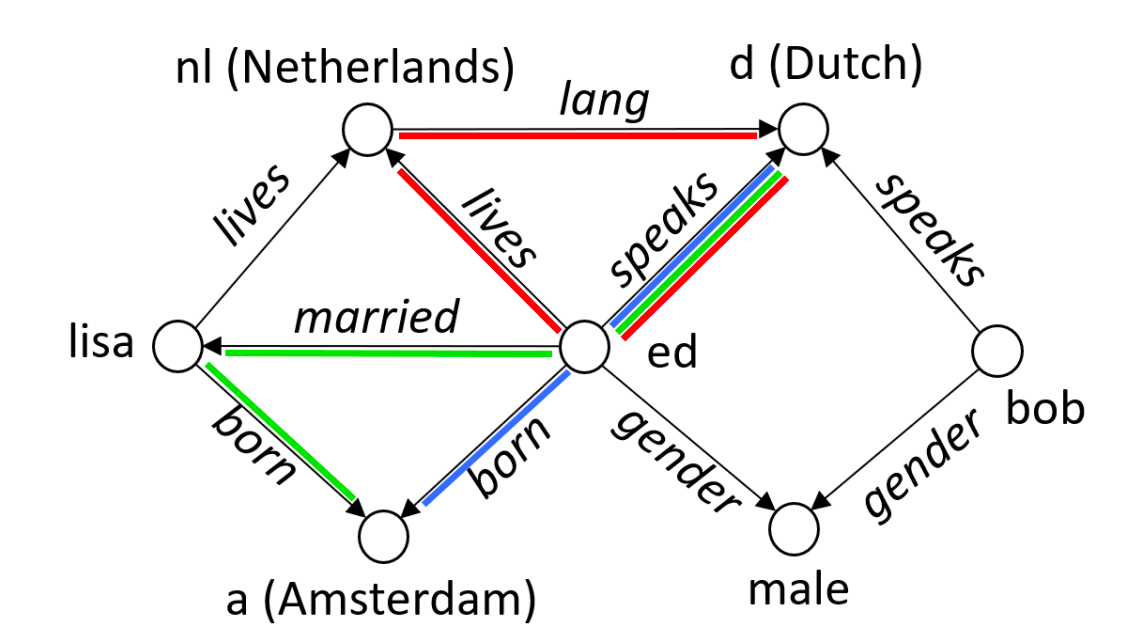
\includegraphics[width=12cm]{images/burl-ago.png}
	\caption{Example of a knowledge graph} 
	\textit{Source: adapted from \href{http://web.informatik.uni-mannheim.de/AnyBURL/2019-05/meilicke19anyburl.pdf}{meilicke19anyburl.pdf}}
	\label{fig:burl}
\end{figure*}

In addition, rules of type \(B\) and \(U_c\) are also referred to as closed-path rules. These are utilized by the AMIE model, described in \cite{AMIE,galarraga2015fast}. Rule \(U_d\) is considered an open rule or an acyclic path rule, since \(A_n\) is a variable that appears only once. For example:



\begin{equation*}
\begin{matrix}
	\textit{speaks}(X, Y ) & \gets & \textit{lives}(X, Y) & \quad (1) \\
	\textit{lives\_in\_city}(X, Y ) & \gets & \textit{lives}(X, A),\textit{within}(Y, A)  & \quad  (2) \\
	\textit{gen}(X, female) & \gets & \textit{married}(X, A), \textit{gen}(A, male)  & \quad  (3) \\
	\textit{profession}(X, actor) &  \gets & \textit{acted\_in}(X, A)  & \quad (4)
\end{matrix}
\end{equation*}


Rule (1) is a \textbf{B}-type rule (binary rule). This rule states that a person (entity) \(X\) speaks language \(Y\) if person \(X\) lives in country \(Y\). Clearly, this is a general rule: whenever entity \(X\) has an edge to entity \(Y\) labeled \textit{lives}, we can infer the existence of another edge labeled \textit{speaks} between \(X\) and \(Y\).

Rules (2) and (3) are both \(U_c\)-type rules. Rule (2) states that a person \(X\) lives in city \(Y\) if person \(X\) lives in country \(A\) and city \(Y\) is located in country \(A\). Rule (3) states that a person \(X\) is female if they are married to person \(A\) and person \(A\) is male. In rule (3), there is no cycle formed in the graph, unlike in rule (2), where node \(Y\) is repeated both in the \textit{head atom} and as the final node in the \textit{body atoms}.

Rule (4) is a \(U_d\)-type rule, which states that a person \(X\) is an actor if they acted in a movie \(A\).

All rules under consideration are filtered based on a score called the rule's confidence, which is computed on the training dataset. This confidence score is defined as the number of \textit{body atom} paths that lead to the \textit{head atom}, divided by the total number of paths that contain only the body atoms.

For example, consider the following rule:  
\(\textit{gen}(X, female) \gets \textit{married}(X, A), \textit{gen}(A, male)\).  
We first count all entity pairs that satisfy the relations \(\textit{married}(X, A), \textit{gen}(A, male)\)—this is the number of paths containing the body atoms. Then we count how many of those pairs also satisfy the inferred relation \(\textit{gen}(X, female)\); this is the number of body atom paths that lead to the head atom. The confidence score of the rule is the ratio of the latter to the former.

\section{AnyBURL Algorithm} \label{myalgorithm}
In this section, we describe the core algorithm of the AnyBURL method, as originally introduced in \cite{burl}, as well as our two extended algorithms designed to handle situations where the graph is incrementally updated with one or more new facts (edges). Additionally, we briefly describe how rules are initialized and how rule confidence is computed using sampling on the training set, including the issue of confidence estimation during prediction when sampling is used.


\subsection{AnyBURL}
\begin{algorithm}
	\caption{Anytime Bottom-up Rule Learning}\label{algorithm1}
	\begin{algorithmic}[1]
		\Procedure{AnyBURL($\mathcal{G}_{\text{know}}$, s, sat, Q, ts)}{}
		\State $\textit{n} = \text{2}$
		\State $R = \emptyset$
		\Loop
		\State $R_s = \emptyset$
		\State $start = currentTime()$
		\Repeat
		\State $p = samplePath(\mathcal{G}_{\text{know}}, n)$
		\State $R_p = generateRules(p)$
		\For {$r \in R_p$}
		\State $score(r, s)$
		\If {$Q(r)$}
		\State $R_s = R_s \cup \{r\}$
		\EndIf
		\EndFor
		\Until {$currentTime() > start + ts$}
		\State $R^{\prime}_s = R_s \cap R$
		\If {$ \mid R^{\prime} \mid / \mid R \mid > SAT$}
		\State $n = n + 1$
		\EndIf
		\State $R = R_s \cap R$
		\EndLoop
		\Return R
		\EndProcedure
	\end{algorithmic}
\end{algorithm}

The input of the algorithm consists of \(\mathcal{G}_{\text{know}}, S, SAT, Q, TS\). The output is the set \(R\) of learned rules. Here, \(\mathcal{G}_{\text{know}}\) is a knowledge graph derived from the training dataset. \(S\) is a parameter indicating the sample size used during each sampling iteration on the training data for confidence computation. \(SAT\) denotes the saturation level of the rules generated in each iteration; this saturation is calculated based on the number of \textbf{new} rules learned in the current iteration relative to the total number of rules already learned. If this value is below the saturation threshold, we consider that there is still potential to discover rules of length \(n\). Otherwise, we increase the rule length and continue the rule mining process. \(Q\) is a threshold used to determine whether a newly generated rule should be added to the result set. \(TS\) indicates the total learning time of the algorithm.

We start with \(n = 2\), which corresponds to rules of path length 2, since a valid path rule requires at least one literal in the head atom and one in the body atoms. In the rule sampling step (\textit{samplePath}), we simply select a random node in the graph, traverse all possible paths from that node with length \(n\), and then randomly select one of the traversed paths.


\subsection{Generate Rules}
\label{subsec:CreateRule}

\begin{algorithm}
	\caption{Generate Rules(p)}
	\label{alg:GenerateRules}
	\begin{algorithmic}[1]
		\Procedure{generate\_rules(p)}{}
		\State $\textit{generalizations} = \emptyset$
		\State $is\_binary\_rule = random.choices([true,false])$
		\If {$is\_binary\_rule$}
		\State $replace\_all\_head\_by\_variables(p)$
		\State $replace\_all\_tail\_by\_variables(p)$
		\State $add(generalizations, p)$
		\Else:
		\State $replace\_all\_head\_by\_variables(p)$
		\State $add(generalizations, p)$
		\State $replace\_all\_tail\_by\_variables(p)$
		\State $add(generalizations, p)$
		\EndIf
		\Return $generalizations$
		\EndProcedure
	\end{algorithmic}
\end{algorithm}

In this algorithm, we substitute constants into the head and tail of all path rules from the sampled rule in the previous step if the rule to be learned is a binary rule. Otherwise, we substitute either the head or the tail and then add the rule to the return set. We then sample a set of rules from the training set and compute their confidence scores as described in \autoref{subsec:CreateRule}. To reduce computational cost, we choose to sample from the training set for this calculation. 

When making predictions for rule candidates, we recompute confidence by incorporating an estimated number of incorrect rules not observed during sampling. For our model, after experimenting with the parameter in the range \([5, 10]\), we found that this yields the best results.

\section{Extended AnyBURL Algorithm}
\subsection{Algorithm 3: Offline-to-Online Learning}


\begin{algorithm}
	\caption{BatchAnyBURL Learning batch size}
	\label{alg:BatchAnyBURL}
	\begin{algorithmic}[1]
		\Procedure{BatchAnyBURL($\mathcal{G}_{know}$, sat, Q, ts, batch\_edge)}{}
		\State $is\_connected = add(\mathcal{G}_{\text{know}}, batch\_edge)$
		\If {$is\_connected$}
		\State  $ G^{\prime} = \mathcal{G}_{\text{know}} \oplus batch\_edge$
		\Else
		\State  $ G^{\prime} = batch\_edge$
		\EndIf
		\State $\textit{n} = \text{2}$
		\State $R = \emptyset$
		\Loop
		\State $R_s = \emptyset$
		\State $start = currentTime()$
		\Repeat
		\State $p = samplePath(G^{\prime}, n)$
		\State $R_p = generateRules(p)$
		\For {$r \in R_p$}
		\State $score(r, G^{\prime})$
		\If {$Q(r)$}
		\State $R_s = R_s \cup \{r\}$
		\EndIf
		\EndFor
		\Until {$currentTime() > start + ts$}
		\State $R^{\prime}_s = R_s \cap R$
		\If {$ \mid R^{\prime} \mid / \mid R \mid > SAT$}
		\State $n = n + 1$
		\EndIf
		\State $R = R_s \cap R$
		\EndLoop
		\Return R
		\EndProcedure
	\end{algorithmic}
\end{algorithm}

This algorithm is our proposed extension to avoid retraining the entire model when a new set of knowledge is added to the graph. When new knowledge is added, we first check whether it is connected to the existing knowledge in the graph (i.e., connectivity). If it is, we perform the \(\oplus\) operation by combining all elements in \(batch\_edge\) with the connected components in the graph, up to a path length of 5. If there is no connectivity, we use all elements in \(batch\_edge\) and repeat the steps of the Anytime Bottom-up Rule Learning algorithm.


\pagebreak

\subsection{Algorithm 4: Online-to-Online Learning}



\begin{algorithm}
	\caption{EdgeAnyBURL}
	\label{alg:EdgeAnyBURL}
	\begin{algorithmic}[1]
		\Procedure{EdgeAnyBURL($\mathcal{G}_{\text{know}}$, s, sat, Q, ts, edge)}{}
		\State $is\_connected = add(\mathcal{G}_{\text{know}}, edge)$
		\State $R = \emptyset$
		\If {$is\_connected$}
		\State $\textit{n} = \text{2}$
		\State $R_s = \emptyset$
		\Repeat
		\State $p = samplePath(edge, n)$
		\State $R_p = generateRules(p)$
		\For {$r \in R_p$}
		\State $score(r, s)$
		\If {$Q(r)$}
		\State $R_s = R_s \cup \{r\}$
		\EndIf
		\EndFor
		\Until {$currentTime() > start + ts$}
		\State $R^{\prime}_s = R_s \cap R$
		\If {$ \mid R^{\prime} \mid / \mid R \mid > SAT$}
		\State $n = n + 1$
		\EndIf
		\State $R = R_s \cap R$
		\EndIf
		\State \Return R
		\EndProcedure
	\end{algorithmic}
\end{algorithm}

This algorithm is a complementary component to \autoref{alg:BatchAnyBURL}. We refer to it as online-to-online because when a new edge (i.e., new knowledge) is added to the graph, we immediately perform learning on the path rules related to that edge—unlike in \autoref{alg:BatchAnyBURL}, where learning is triggered only after a sufficient amount of new knowledge has been added.
